
\documentclass[a4paper,twoside,notitlepage]{article}

\setlength{\oddsidemargin}{2mm}
\setlength{\evensidemargin}{2mm}
\setlength{\textwidth}{154mm}
\setlength{\textheight}{220mm}
\setlength{\topmargin}{0mm}
\setlength{\parskip}{1mm}
\renewcommand{\floatpagefraction} {0.99}
\renewcommand{\textfraction} {0.0}
\renewcommand{\topfraction} {0.99}

\hfuzz=10pt

\vbadness=10001 % the hell with underfull vboxes
\hbadness=10001

\usepackage{etex}
\usepackage{float}
\usepackage{longtable}
\usepackage{tabularx}
\usepackage{graphicx} 
\usepackage[bitheight=6ex]{bytefield}
\usepackage{gensymb}
\usepackage[stable]{footmisc}
\usepackage{multirow}
\usepackage{siunitx}
\usepackage{fancyhdr}
\usepackage[colorlinks=true, pdfstartview=FitV, linkcolor=blue, 
	    citecolor=blue, urlcolor=blue]{hyperref}
\usepackage[dvipsnames]{xcolor}

\usepackage{listings} % Required for inserting code snippets

\usepackage[justification=centering]{caption}
\usepackage{pgfgantt}
\usepackage{tikz-timing}
\usepackage{makecell}
\usepackage{lipsum}

\renewcommand*{\familydefault}{\sfdefault}
%\renewcommand*{\familydefault}{\rmdefault}
%\renewcommand*{\familydefault}{\ttdefault}
%\renewcommand*{\familydefault}{\rmdefault{ppl}}

\makeatletter
\newcommand*{\toccontents}{\@starttoc{toc}}
\makeatother

\begin{document}

\title{\textbf{Marantz PM8006} amplifier repair}
\author{author: Petre Rodan}
\date{revised \today}
\maketitle

%\begin{figure}
%\begin{tabular}{ c p{7cm} }
%
%    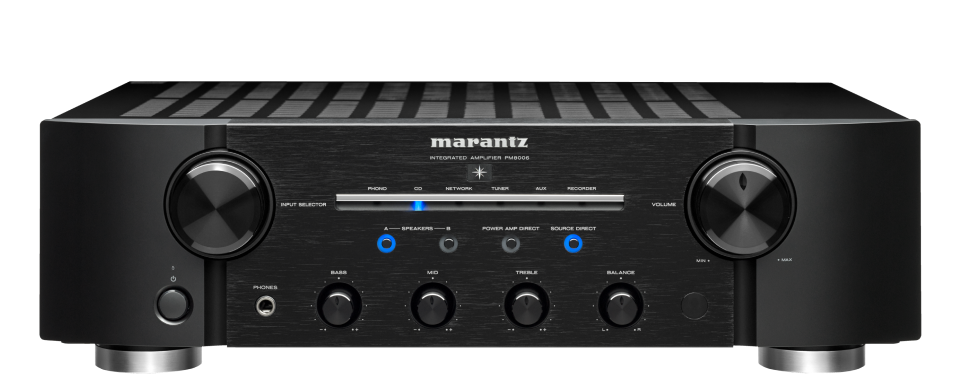
\includegraphics[width=77mm]{img_report/PM8006}} &
%    \textbf{Description:} distorsion is heard on left channel of the amplifier whenever sound is played, and it dissapears if there is no audio signal on the input.
%    an electrical and thermal analysis is run on the unit in order to detect the source of the problem

%\end{tabular}
%\end{figure}

%\tableofcontents
\toccontents

\section{problem overview} \label{sec:problem-overview}

distorsion is heard on the left channel of the amplifier whenever sound is played, and it dissapears if there is no audio signal present.

the distorsion is not present immediately after the mixer/selector/tone control stages, so the problem is clearly further down the audio path. there is a negative feedback (NFB) link between the power amp and the main pcbs via pin 5 of the B6001 connector (see schematic in Fig \ref{fig:waveform-testpoints}), so both these pcbs have to be analyzed to understand where the source of the problem is located.

one very hot (90+\si{\celsius}) transistor (Q7009) is located on power amplifier board. due to assembly constraints, the power pcb is reachable only after taking the amplifier apart. so testing will start with the main pcb, while the amp can be kept powered on and all pcbs in-situ.

power amp rail voltages are ±50V with no load (documentation specifies ±46.6V).

as a test signal, a \SI{1}{\kilo\hertz} \SI{500}{\milli\volt} pkpk signal is fed into 'Point A' of both channels. dummy loads (9.4\si{\ohm} ea.) are present on both speaker outputs.

\clearpage
\section{main pcb. waveform measurements} \label{sec:waveform-measurements}

a number of testpoints have beed selected on the main board in order to compare the signals between the working (right) channel and the distorted (left) one. the scope signals are presented below.

\begin{figure}[hptb!]
    \centering
    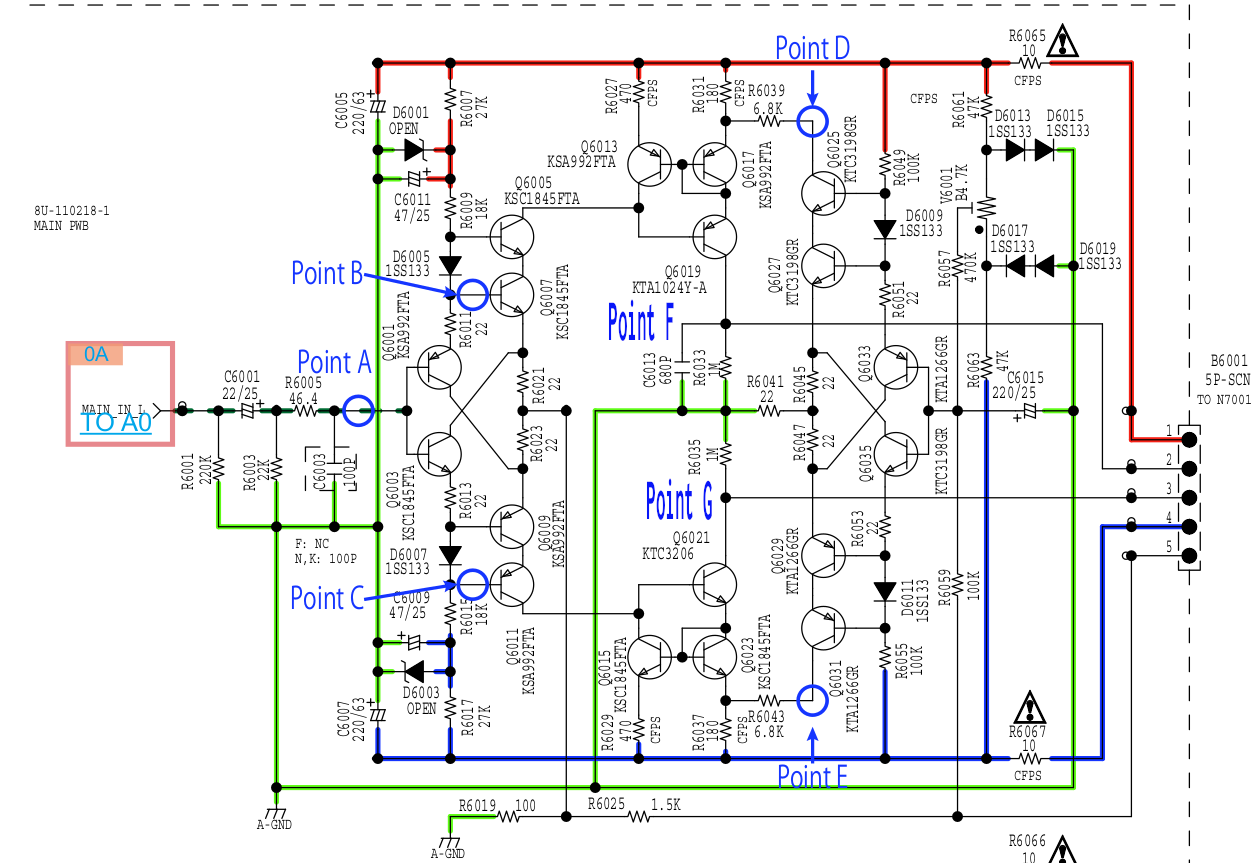
\includegraphics[width=12cm]{img_report/waveform_testpoints}
 \caption{main pcb left channel, waveform testpoints}
 \label{fig:waveform-testpoints}
\end{figure}

\begin{figure}[hptb!]
    \centering
    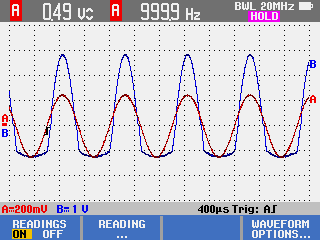
\includegraphics[width=6cm]{img_report/left_point_A.png}
    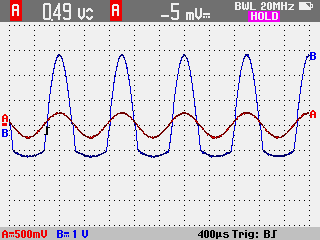
\includegraphics[width=6cm]{img_report/right_point_A.png} \\ 
    \textcolor{Red}{red signal} - Point A on left and right channels respectively \\
    \textcolor{Blue}{blue signal} - left channel output (on both plots) \\
    note: signals are identical (500mV pkpk, no DC offset)
 \caption{Point A}
 \label{fig:point-A}
\end{figure}

\begin{figure}[hptb!]
    \centering
    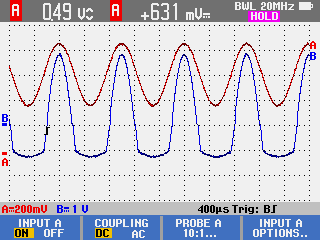
\includegraphics[width=6cm]{img_report/left_point_B.png}
    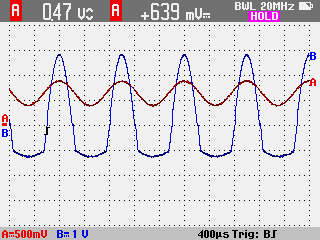
\includegraphics[width=6cm]{img_report/right_point_B.png} \\ 
    \textcolor{Red}{red signal} - Point B on left and right channels respectively \\
    \textcolor{Blue}{blue signal} - left channel output (on both plots) \\
    note: signals are identical (500mV pkpk, +630mV DC offset)
 \caption{Point B}
 \label{fig:point-B}
\end{figure}

\begin{figure}[hptb!]
    \centering
    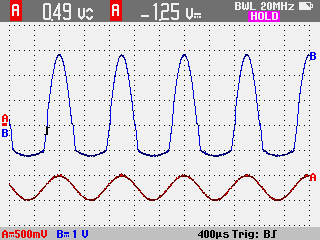
\includegraphics[width=6cm]{img_report/left_point_C.png}
    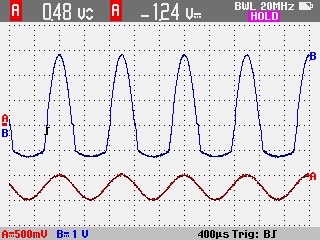
\includegraphics[width=6cm]{img_report/right_point_C.png} \\ 
    \textcolor{Red}{red signal} - Point C on left and right channels respectively \\
    \textcolor{Blue}{blue signal} - left channel output (on both plots) \\
    note: signals are identical (500mV pkpk, -1.25V DC offset)
 \caption{Point C}
 \label{fig:point-C}
\end{figure}

\begin{figure}[hptb!]
    \centering
    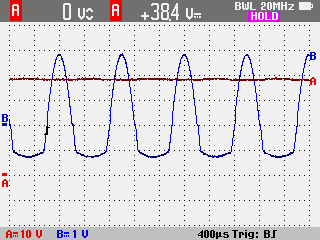
\includegraphics[width=6cm]{img_report/left_point_D.png}
    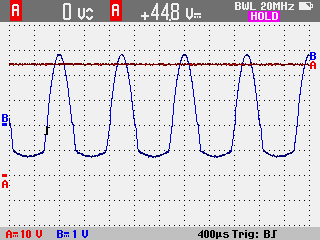
\includegraphics[width=6cm]{img_report/right_point_D.png} \\ 
    \textcolor{Red}{red signal} - Point D on left and right channels respectively \\
    \textcolor{Blue}{blue signal} - left channel output (on both plots) \\
    note: signals are not identical (0V pkpk, 38V/45V DC offset)
 \caption{Point D}
 \label{fig:point-D}
\end{figure}

\begin{figure}[hptb!]
    \centering
    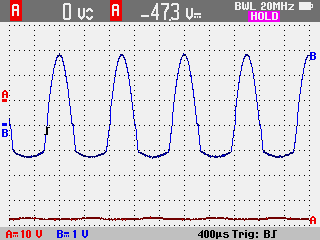
\includegraphics[width=6cm]{img_report/left_point_E.png}
    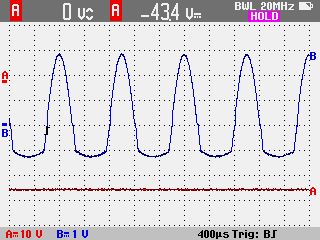
\includegraphics[width=6cm]{img_report/right_point_E.png} \\ 
    \textcolor{Red}{red signal} - Point E on left and right channels respectively \\
    \textcolor{Blue}{blue signal} - left channel output (on both plots) \\
    note: signals are not identical (0V pkpk, -47V/-43V DC offset)
 \caption{Point E}
 \label{fig:point-E}
\end{figure}

\begin{figure}[hptb!]
    \centering
    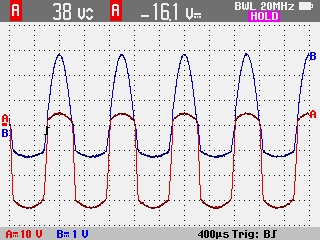
\includegraphics[width=6cm]{img_report/left_point_F.png}
    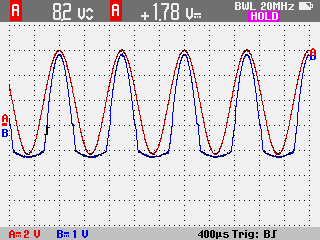
\includegraphics[width=6cm]{img_report/right_point_F.png} \\ 
    \textcolor{Red}{red signal} - Point F on left and right channels respectively \\
    \textcolor{Blue}{blue signal} - left channel output (on both plots) \\
    note: signals are not identical (38V/8V pkpk, -16V/+1.8V DC offset)
 \caption{Point F}
 \label{fig:point-F}
\end{figure}

\begin{figure}[hptb!]
    \centering
    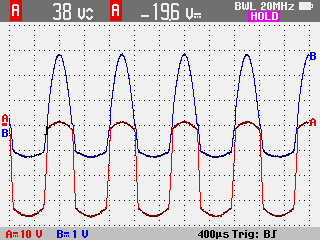
\includegraphics[width=6cm]{img_report/left_point_G.png}
    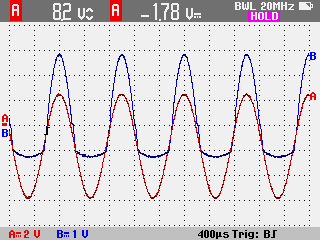
\includegraphics[width=6cm]{img_report/right_point_G.png} \\ 
    \textcolor{Red}{red signal} - Point G on left and right channels respectively \\
    \textcolor{Blue}{blue signal} - left channel output (on both plots) \\
    note: signals are not identical (38V/8V pkpk, -19V/-1.8V DC offset)
 \caption{Point G}
 \label{fig:point-G}
\end{figure}

\begin{figure}[hptb!]
    \centering
    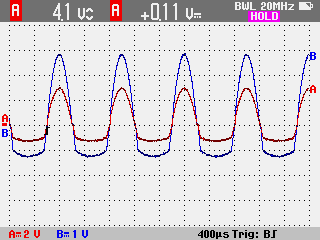
\includegraphics[width=6cm]{img_report/left_NFB.png}
    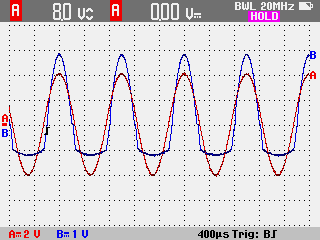
\includegraphics[width=6cm]{img_report/right_NFB.png} \\ 
    \textcolor{Red}{red signal} - NFB signal left and right channels respectively \\
    \textcolor{Blue}{blue signal} - left channel output (on both plots) \\
 \caption{negative feedback signals}
 \label{fig:NFB}
\end{figure}

\begin{figure}[hptb!]
    \centering
    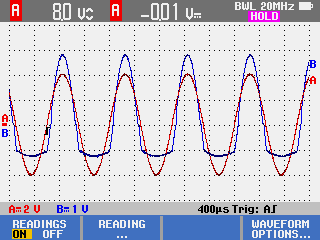
\includegraphics[width=6cm]{img_report/outputs_broken.png} \\
    \textcolor{Red}{red signal} - right channel output \\
    \textcolor{Blue}{blue signal} - left channel output \\
 \caption{speaker output signals}
 \label{fig:output}
\end{figure}

\clearpage
\section{main pcb. DC measurements} \label{sec:dc-measurements}

\begin{figure}[hptb!]
    \centering
    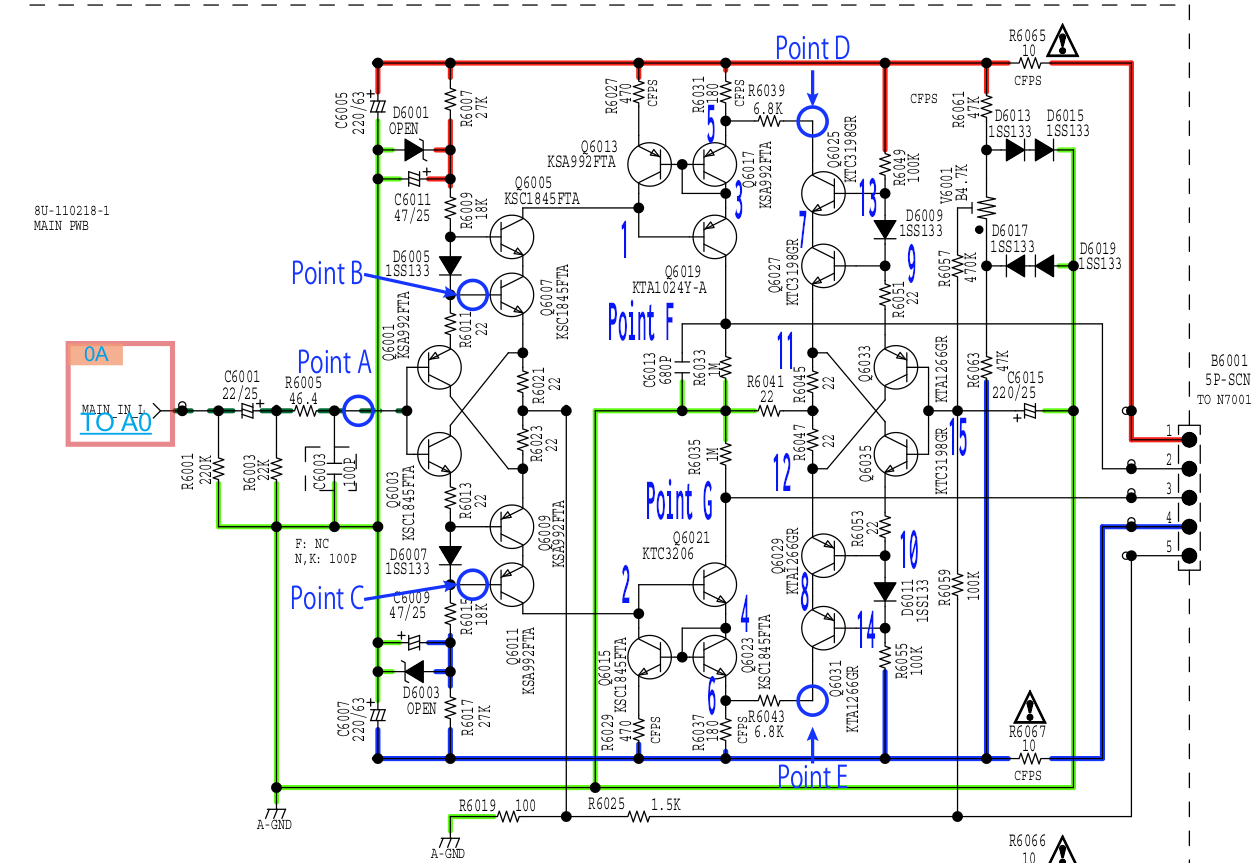
\includegraphics[width=12cm]{img_report/dc_testpoints}
 \caption{main pcb left channel, dc testpoints}
 \label{fig:dc-testpoints}
\end{figure}

\begin{table}[hptb!]
\centering
\begin{tabular}{ c | c | c }
    point & R ch & L ch\\ \hline
    1 & 46.5 & 47.2 \\
    2 & -47 & -47.4 \\
    3 & 47.3 & 47.7 \\
    4 & -47.7 & -48 \\
    5 & 48.4 & 48.6 \\
    6 & -48.2 & -48.2 \\
    7 & 0.6 & 0.65 \\
    8 & -0.6 & -0.5 \\
    9 & 0.6 & 0.7 \\
    10 & -0.6 & -0.5 \\
    11 & 0 & 0 \\
    12 & 0 & 0 \\
    13 & 1.1 & 1.23 \\
    14 & -1.2 & -1.1 \\
    15 & 0 & 0 \\
 \end{tabular}
 \caption{main pcb left channel, dc testpoint measurements}
 %\caption{dc testpoint measurements}
 \label{tab:dc-testpoints-meas}
\end{table}

\clearpage
\section{main pcb. thermal measurements} \label{sec:thermal-measurements}

% right channel

\begin{figure}[hptb!]
 \centering
 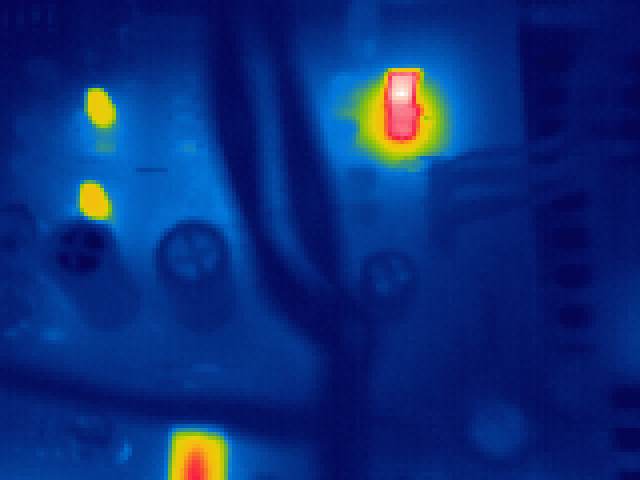
\includegraphics[height=8cm, keepaspectratio=true]{img_report/IR_6353}
 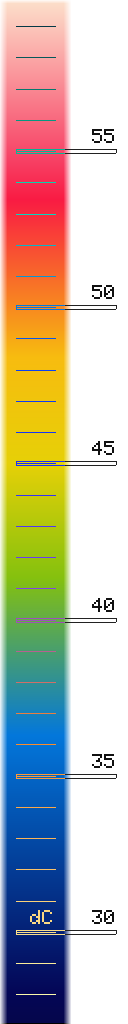
\includegraphics[height=8cm, keepaspectratio=true]{img_report/IR_6353_scale}
 \label{fig:left-ch-ir}

 \vspace*{5mm}
 \begin{tabular}{ l | l }
  Label & Value \\ \hline
  IR: File Name & IR\_6353.jpg \\
  IR: Max & 59.84 C \\
  emissivity & 0.95 \\
  img create date & 2021:12:15 17:16:43 \\
 \end{tabular}
 \caption{main pcb right channel - Q6022 (KTC3206) and Q6020 (KTA1024Y-A) have elevated temperatures (55\si{\celsius})}
\end{figure}

\begin{figure}[hptb!]
 \centering
 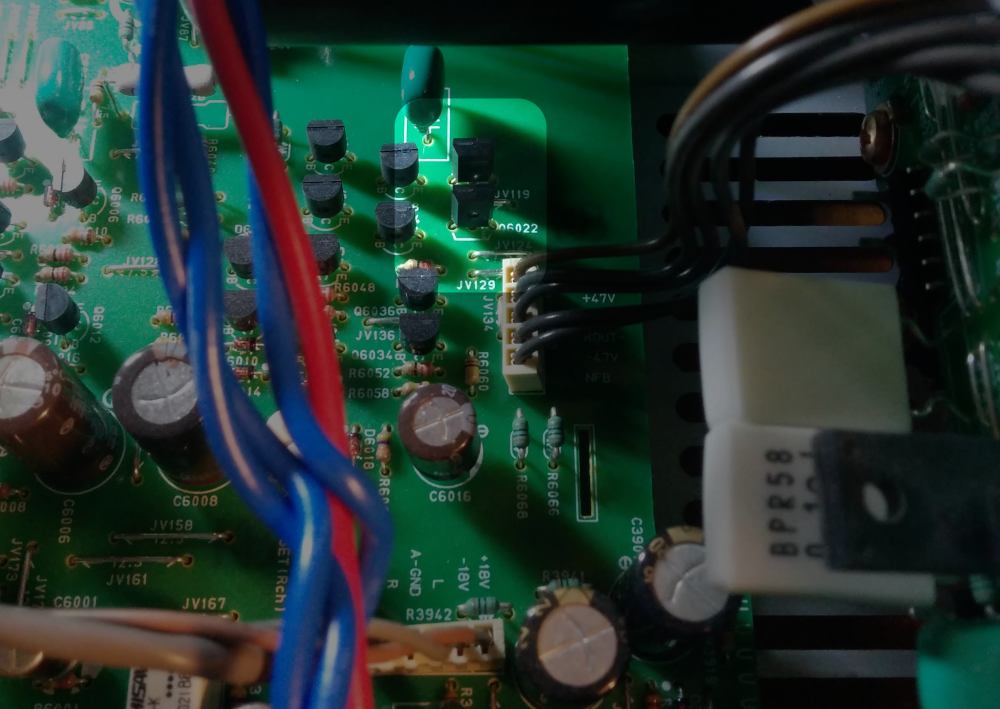
\includegraphics[width=7cm, keepaspectratio=true]{img_report/main_pcb_r.png}
 \caption{photo of the Q6022 and Q6020 transistors}
\end{figure}


% left channel

\begin{figure}[hptb!]
 \centering
 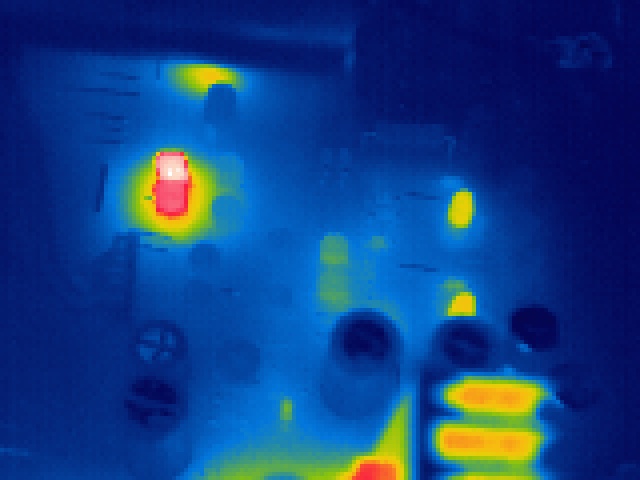
\includegraphics[height=8cm, keepaspectratio=true]{img_report/IR_6352}
 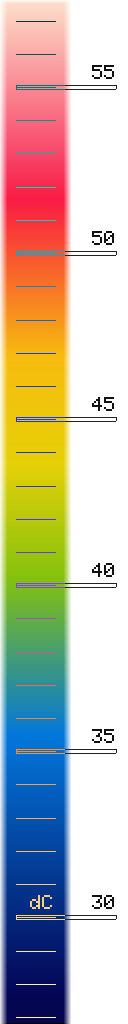
\includegraphics[height=8cm, keepaspectratio=true]{img_report/IR_6352_scale}

 \vspace*{5mm}
 \begin{tabular}{ l | l }
  Label & Value \\ \hline
  IR: File Name & IR\_6352.jpg \\
  IR: Max & 57.62 C \\
  emissivity & 0.95 \\
  img create date & 2021:12:15 17:16:15
 \end{tabular}
 \caption{main pcb left channel - Q6021 (KTC3206) and Q6019 (KTA1024Y-A) getting above 50\si{\celsius}}
 \label{tab:main-pcb-l-ir}
\end{figure}

\begin{figure}[hptb!]
\centering
 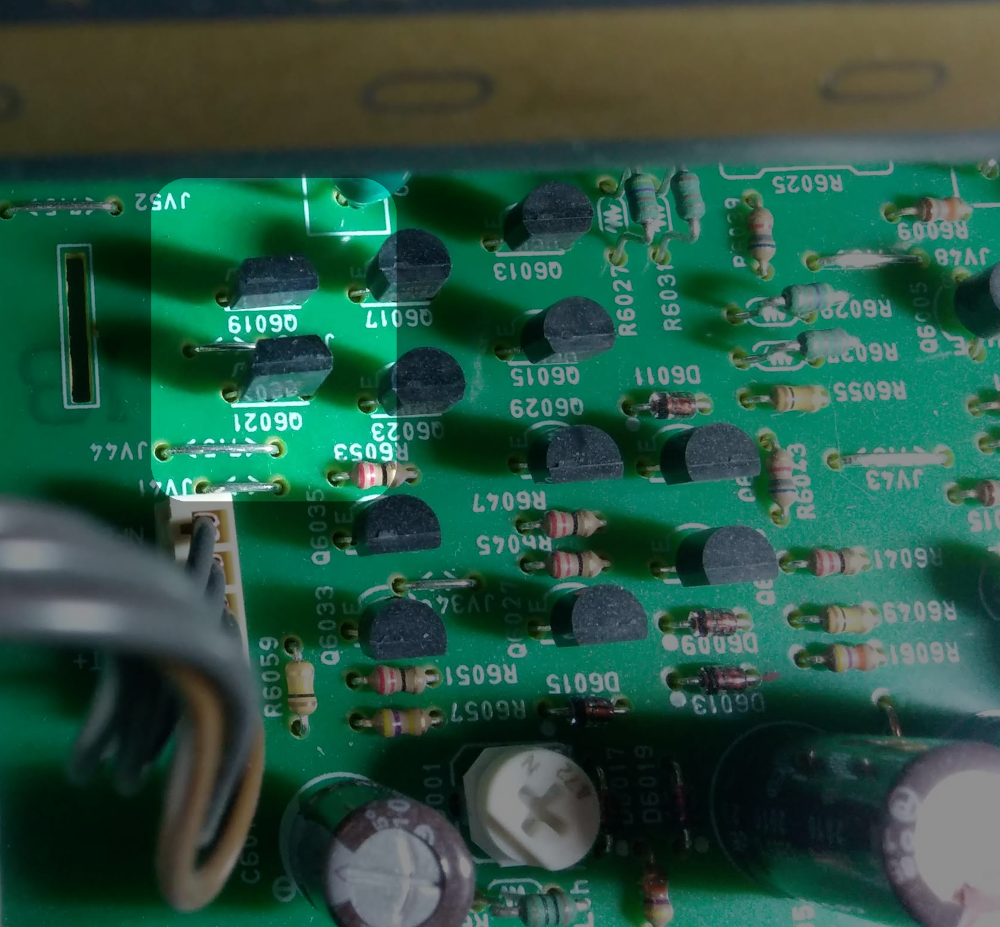
\includegraphics[width=6.8cm, keepaspectratio=true]{img_report/main_pcb_l.png}
 \caption{photo of the Q6021 and Q6019 transistors}
\end{figure}

\clearpage
\section{power amp pcb. thermal measurements} \label{sec:pwr-thermal-measurements}

% right channel

\begin{figure}[hptb!]
 \centering
 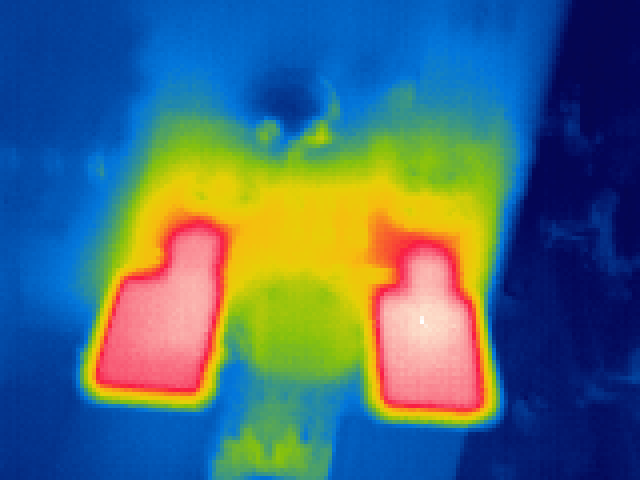
\includegraphics[height=8cm, keepaspectratio=true]{img_report/IR_6348}
 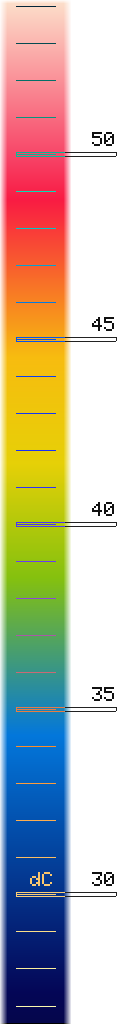
\includegraphics[height=8cm, keepaspectratio=true]{img_report/IR_6348_scale}
 \label{fig:pwr-left-ch-ir}

 \vspace*{5mm}
 \begin{tabular}{ l | l }
  Label & Value \\ \hline
  IR: File Name & IR\_6348.jpg \\
  IR: Max & 54.15 C \\
  emissivity & 0.95 \\
  img create date & 2021:12:15 15:35:01 \\
 \end{tabular}
 \caption{power amp pcb right channel - driver transistors have similar temperatures on this channel (53\si{\celsius})}
\end{figure}

\begin{figure}[hptb!]
 \centering
 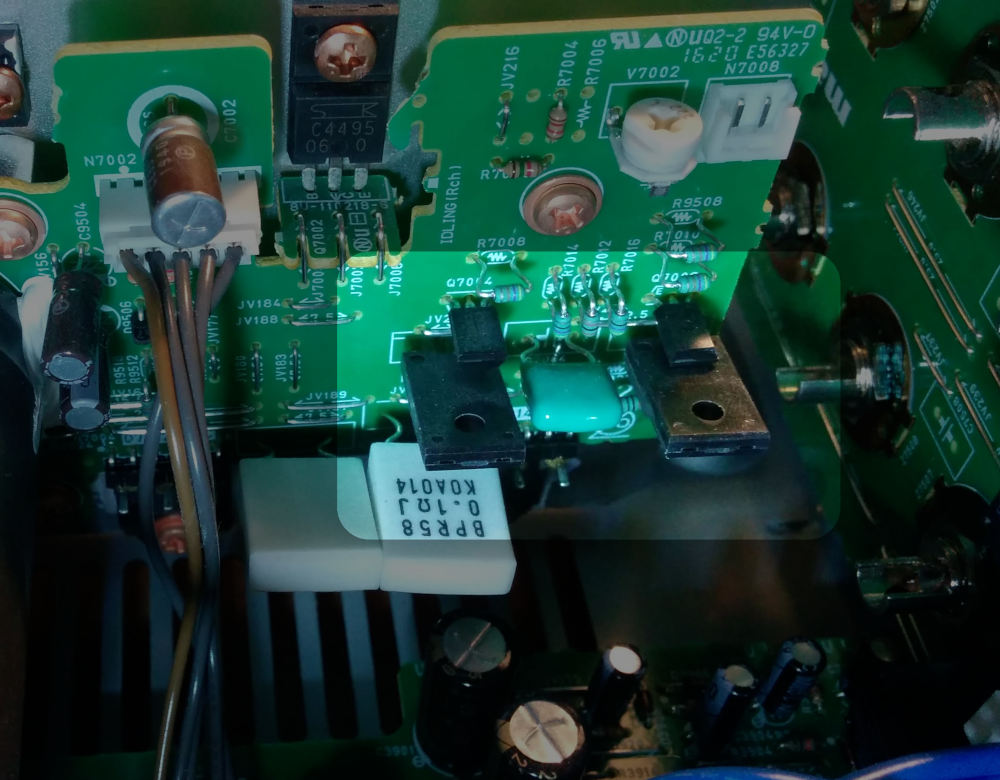
\includegraphics[width=7cm, keepaspectratio=true]{img_report/power_amp_pcb_r.png}
 \caption{photo of the Q6022 and Q6020 transistors}
\end{figure}


% left channel

\begin{figure}[hptb!]
 \centering
 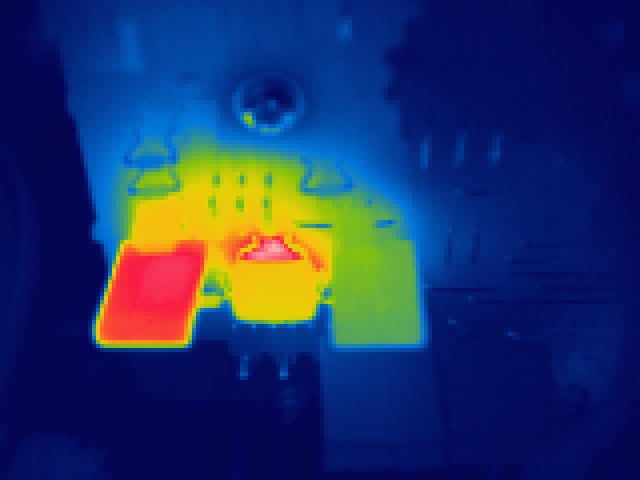
\includegraphics[height=8cm, keepaspectratio=true]{img_report/IR_6357}
 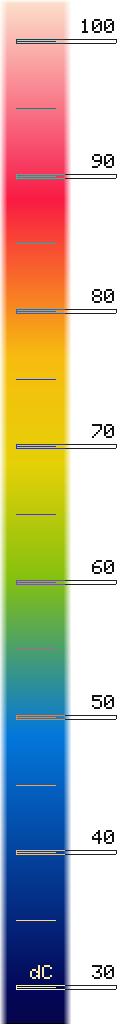
\includegraphics[height=8cm, keepaspectratio=true]{img_report/IR_6357_scale}

 \vspace*{2mm}
 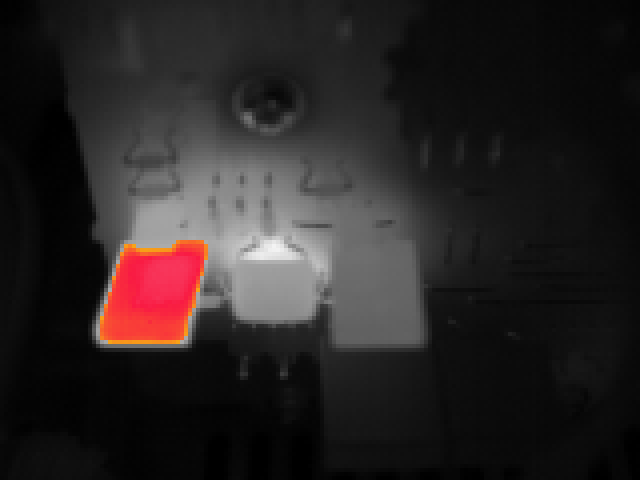
\includegraphics[height=4.36cm, keepaspectratio=true]{img_report/q7009}
 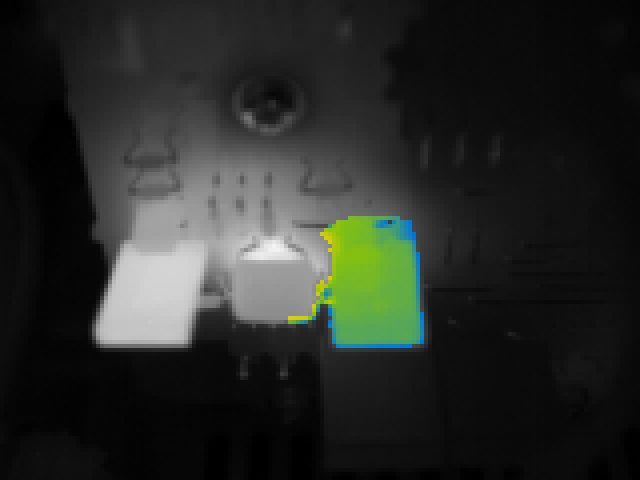
\includegraphics[height=4.36cm, keepaspectratio=true]{img_report/q7007}

 \vspace*{5mm}
 \begin{tabular}{ l | l }
  Label & Value \\ \hline
  IR: File Name & IR\_6357.jpg \\
  IR: Max & 98.91 C \\
  emissivity & 0.95 \\
  img create date & 2021:12:15 17:22:37 \\
  Q7009 max & 90.08 C !!! \\
  Q7007 max & 60.20 C \\
 \end{tabular}

 \caption{power amp pcb left channel - large temperature delta between Q7009 and Q7007}
 \label{tab:pwr-pcb-l-ir}
\end{figure}

\begin{figure}[hptb!]
\centering
 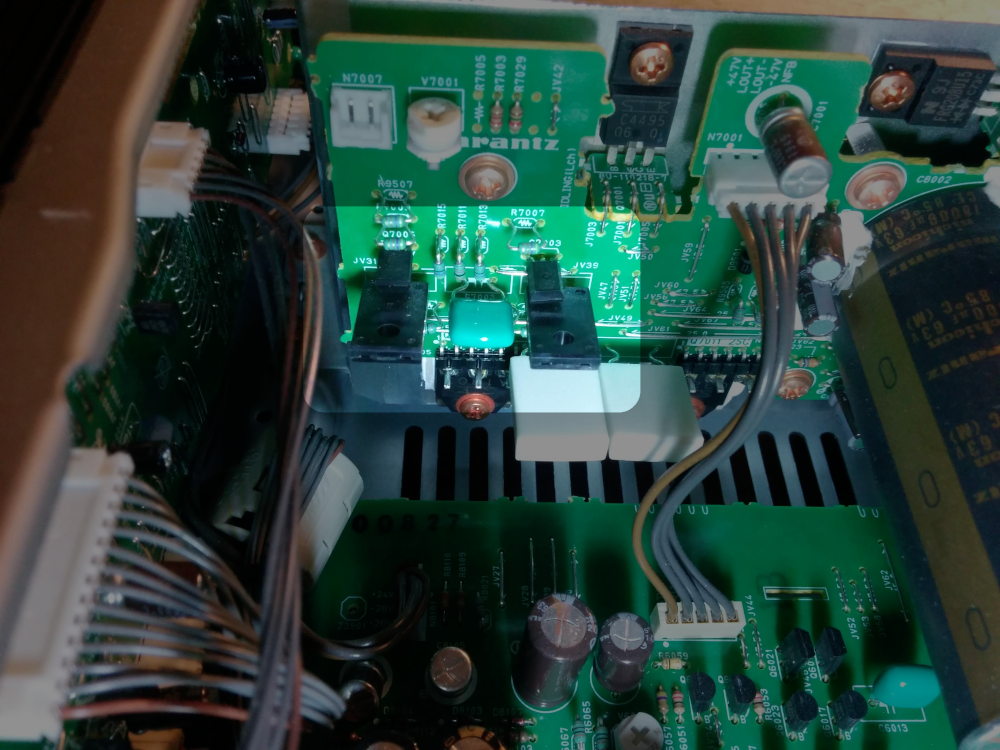
\includegraphics[width=6.8cm, keepaspectratio=true]{img_report/power_amp_pcb_l}
 \caption{photo of the Q6021 and Q6019 transistors}
\end{figure}

despite the large temperature difference between the two driver transistors of the left channel, all PN junctions measured correctly.

since no actual fault has been detected up until now on the main pcb, the presumption is made that the detected distorsion is caused by the negative feedback signal and probably the fault lies in the power amp pcb, which needs to be completely extracted from the amplifier and thus cannot be probed while under load.

once the power amp pcb was extacted, it was clear that Q7013, one of the final power transistor of the let channel had it's base floating due to a cold solder joint (see Fig \ref{fig:q7013}).

once the connection was fixed the distorsion has dissapeared and all temperatures came back to normal on the left channel.

\begin{figure}[hptb!]
\centering
 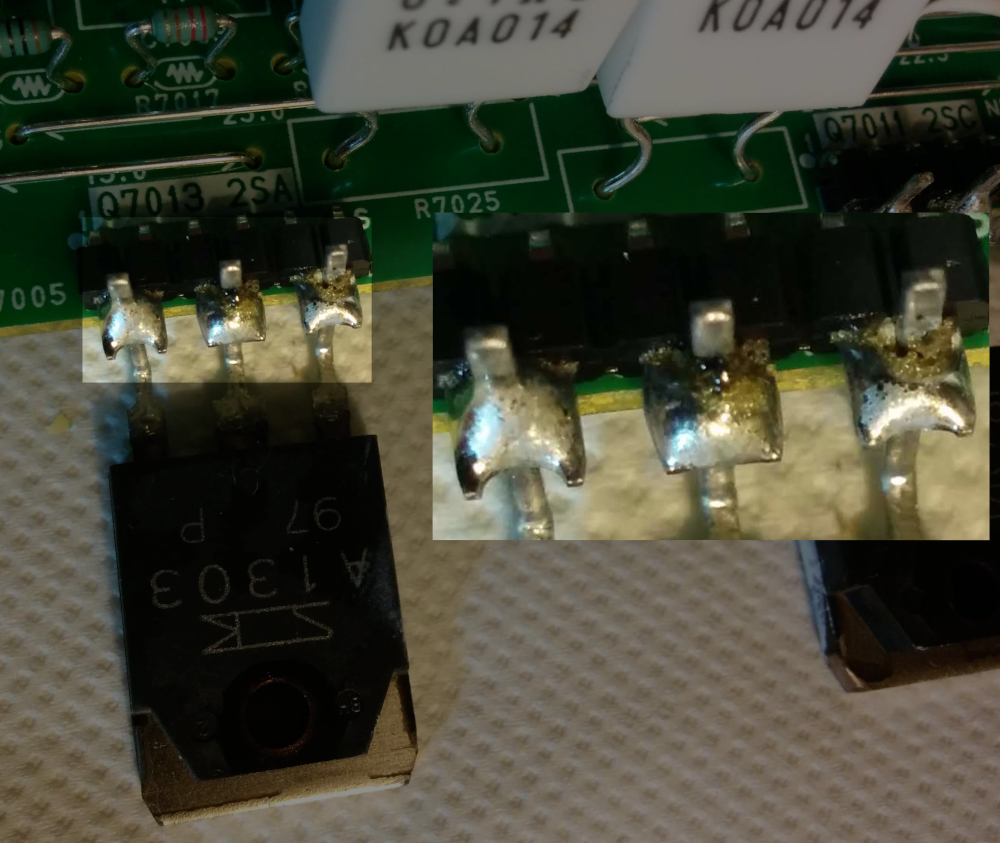
\includegraphics[width=6.8cm, keepaspectratio=true]{img_report/q7013}
 \caption{photo of the Q7013 transistor on the power amp pcb}
 \label{fig:q7013}
\end{figure}

\begin{figure}[hptb!]
 \centering
 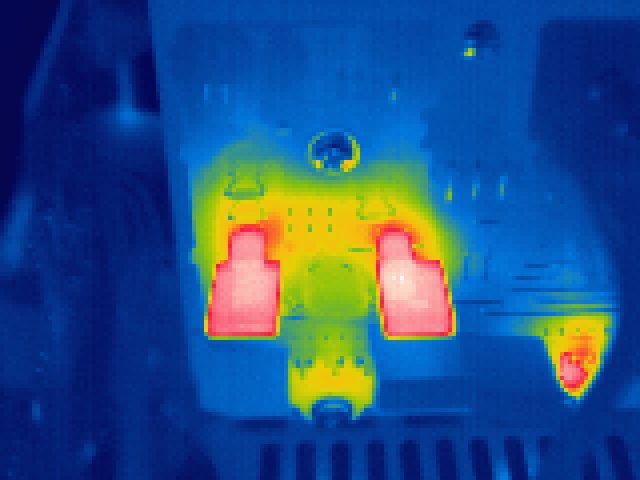
\includegraphics[height=8cm, keepaspectratio=true]{img_report/IR_6361}
 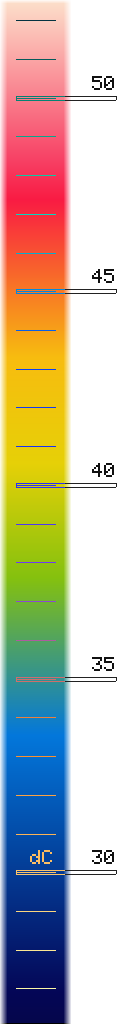
\includegraphics[height=8cm, keepaspectratio=true]{img_report/IR_6361_scale}

 \vspace*{5mm}
 \begin{tabular}{ l | l }
  Label & Value \\ \hline
  IR: File Name & IR\_6361.jpg \\
  IR: Max & 52.52 C \\
  emissivity & 0.95 \\
  img create date & 2021:12:17 07:34:55
 \end{tabular}

 \caption{power amp pcb left channel after repair - Q7009 and Q7007 at the same temperature}
\end{figure}

\begin{figure}[hptb!]
 \centering
 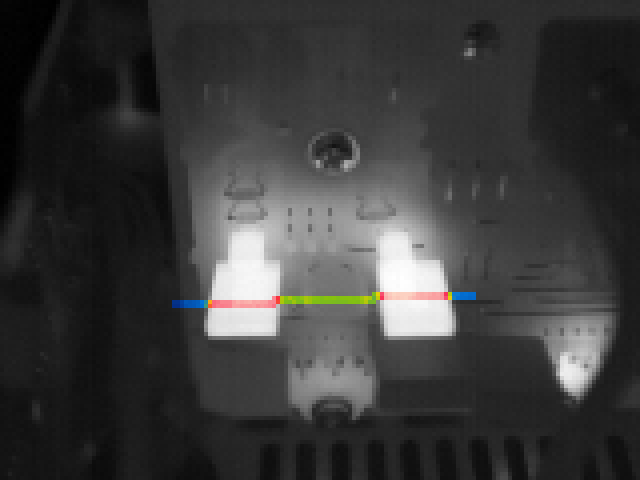
\includegraphics[height=8cm, keepaspectratio=true]{img_report/IR_6361_hl}
 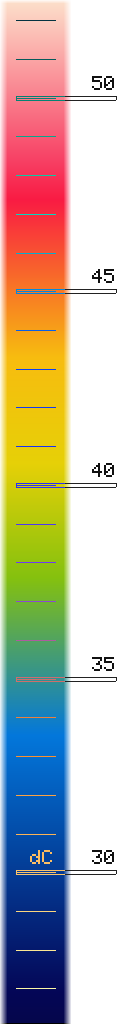
\includegraphics[height=8cm, keepaspectratio=true]{img_report/IR_6361_scale}

 \vspace*{5mm}
 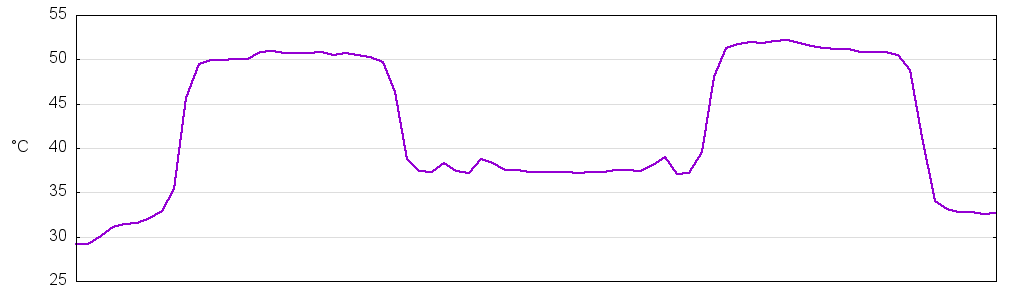
\includegraphics[width=12cm, keepaspectratio=true]{img_report/IR_6361_hl_gnuplot}

 \caption{power amp pcb left channel after repair - Q7009 and Q7007 at the same temperature}
\end{figure}

\begin{figure}[hptb!]
 \centering
 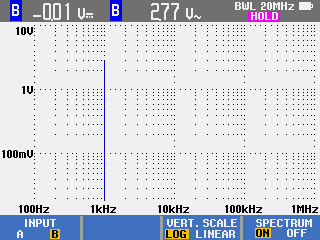
\includegraphics[width=6cm, keepaspectratio=true]{img_report/output_L_fft.png}
 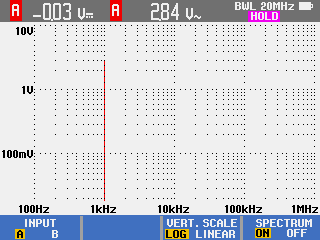
\includegraphics[width=6cm, keepaspectratio=true]{img_report/output_R_fft.png}

 \vspace*{5mm}
 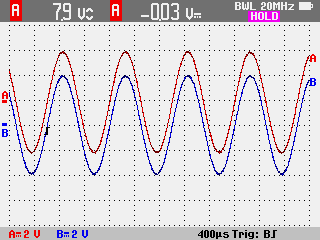
\includegraphics[width=6cm, keepaspectratio=true]{img_report/outputs_repaired.png}

 \textcolor{Red}{red signal} - right channel output \\
 \textcolor{Blue}{blue signal} - left channel output \\

 \caption{output signals and fft plots after the repair}
\end{figure}




\end{document}
